\chapter{Methods}\label{methods}

For this project, I am interested in two factors that help characterise the cancer mutation profile: genomic location effect (GLE) and sequence context effect (SCE; Figure \ref{fig:workflow}). I examined each factor on two complementary scales: analysis of whole disease (section \ref{methods:gle} and \ref{methods:sce}) and cancer classification for individuals (section \ref{methods:ml}). The former somewhat plays the role of a biological basis for the latter, whereas the latter could validate the patterns detected by the former.

\begin{figure}[h!]
    \centering
    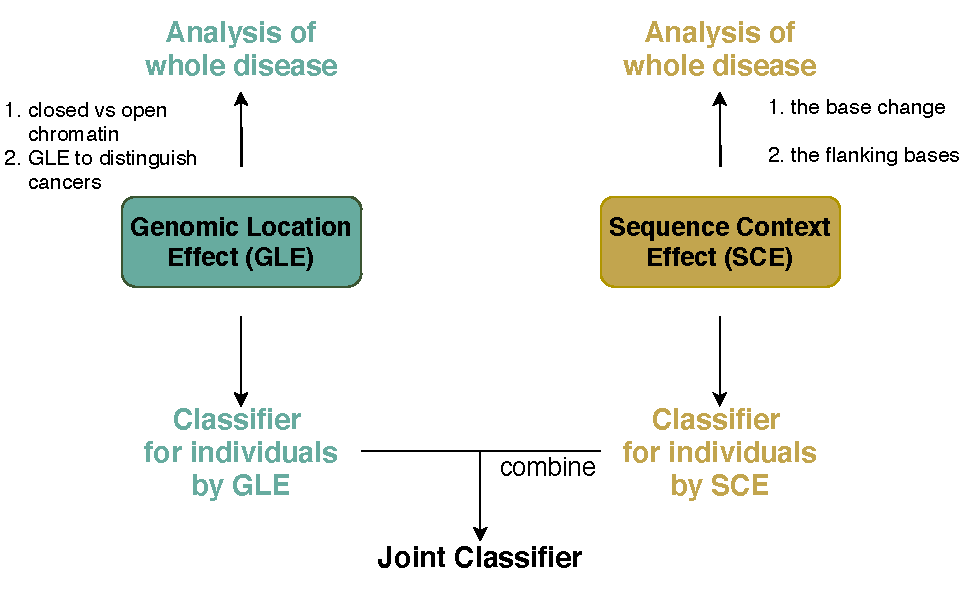
\includegraphics[scale=0.85]{graphics/workflow.pdf}
\caption{}
    % \caption{\textbf{Project workflow for understanding cancer mutagenesis data and exploiting it for cancer classification.} On one hand, cancers were analysed on the whole disease scale, which considered mutations from all donors of the same diseases as a whole. This magnified the signals in the data and made it easier for understanding the mutagenesis process. On the other hand, the information from the factors analysed above was used for training a classifier on the individual donor scale, meaning that this classifier could potentially be applied to a new patient's mutation data to predict their cancer. This followed a standard machine learning training procedure, outlined in Section \ref{methods:ml}.}
    \label{fig:workflow}
\end{figure}


\section{Data description}
\subsection{PCAWG - Mutation data:} 
The critical source of data for the project is the Pan-Cancer Analysis of Whole Genome (PCAWG) project \citep{Campbell2020}. This data consists of whole genome sequencing of both cancerous and healthy tissues (mostly blood) for all cancer patients. PCAWG relies on contrasting the cancerous against healthy tissues to determine whether a mutation is a \gls{sommut}. Identifying mutations by combining three established pipelines (Sanger \citep{Jones2016CgpCaVEManWrapper:Data}, EMBL/DKFZ \citep{Rimmer2014IntegratingApplications}, and Broad \citep{Cibulskis2013SensitiveSamples}), the project provides a valuable resource, which covers 2658 cancer samples from 28 cancer types, for studying cancer mutagenesis.

This project is limited to somatic \glspl{point_mut}. I sampled 12 cancers whose DHS data for the putative original cells is also available (Table \ref{tab:encode}). A summary of the mutations for the 12 cancers can be found in the appendix Table \ref{tab:mutation_summary} and Figure \ref{fig:mutation_summary}. Mutation data for all individuals and all mutations was downloaded as a MAF file from the \href{https://dcc.icgc.org/releases/PCAWG/consensus_snv_indel}{International Cancer Genome Consortium (ICGC)}. Driver mutations were then filtered out based on \href{https://dcc.icgc.org/releases/PCAWG/driver_mutations}{the PCAWG's driver mutation project} because driver mutations are under selection pressure and have different mutation rates to passenger mutations. The information this project utilised from PCAWG was the mutations, their genomic locations, their donor ID and the donor's cancer. 

\subsection{Reference genome:} 
To reconstruct the cancer genome, both mutation data and a standard human reference genome are required. The human reference genome was provided by Ensembl \citep{Yates2020Ensembl2020}, and downloaded from the \href{http://hgdownload.soe.ucsc.edu/goldenPath/hg19/chromosomes}{UCSC genome browser}. As PCAWG used Human Genome Assembly 37, the same version of genomic coordinates is used for this project. As an additional check, I also assert that the wildtype base at each mutated position and its local reference sequence context provided by PCAWG match the sequence at that position from the reference genome. 

\subsection{Chromatin status data:} 
Part of my project investigates the relationship between mutation distribution and chromatin status. Based on literature search, I identified the most likely tissue of origin for the cancer of interest, summarised in Table \ref{tab:encode}. DNase I hypersensitivity (DHS) data for these tissues of origin, as a canonical measure for chromatin status, was provided by ENCODE \citep[downloaded from either \href{https://genome.ucsc.edu/cgi-bin/hgFileUi?db=hg19&g=wgEncodeOpenChromDnase}{Duke} or \href{https://genome.ucsc.edu/cgi-bin/hgFileUi?db=hg19&g=wgEncodeUwDnase}{UW};][]{Thurman2012TheGenome,Klemm2019ChromatinEpigenome}. Specifically, ENCODE measured the level of Dnase hypersensitivity across the genome and identified Dnase hypersensitive regions based on an established threshold. Here, open chromatin regions are defined as the Dnase hypersensitive range and closed chromatin regions are the rest of the genome. The relationship between the original cells based on DHS can be visualised in Figure \ref{fig:encode_pca} via the multiple dimension scaling technique (details in Subsection \ref{methods:encode_pca}). 

\section{Algorithm development}
\subsection{Reproducibility} 
\href{http://git-scm.com}{Git} was used as a Version Control tool. Accordingly, the entire code history has been recorded and stored on \href{https://github.com}{GitHub}.

The entire project was done in loops, which means that most analyses were repeated on increasing scales. This not only increases the opportunity for code efficiency to be improved but also helps ensure that the algorithms are reproducible. 

While the project is too large to be shared in a thesis, all code is available upon request. 

\subsection{Developing packages}
Most core functions were written in Python \citep{van1995python}, with visualisation and some analyses written in R \citep{r}. Code was written as packages that can be installed and utilised by anyone with the permission. 

All core functions were tested under explicit hypothetical scenarios for correctness before being applied. This process is called unit testing. Each of the analyses requires multiple core functions. For each analysis, core functions are combined in one \href{https://click.palletsprojects.com/en/8.0.x/}{click} command that can be run either in the command line or conventional Python platforms such as Jupyter Notebook. The \href{https://github.com/HuttleyLab/scitrack}{Scitrack} Python package was applied to these commands so that not only code, but inputs and outputs of these commands were tracked as well.

\subsection{Parallelisation}
When analysing large data sets, some steps could be considerably time-consuming, particularly the initial data filtering step and the simulation steps. Therefore, for several steps, I have written scripts that optimise code parallelisation based on the original command line. By doing this, for an analysis that executes the same processes multiple times on independent objects, these objects were ``distributed'' into different computer cores instead of being processed sequentially on one single computer. This was supported by the National Computational Infrastructure Australia.


\section{Whole disease analysis of GLE}\label{methods:gle}

The variation in chromatin structures of different cell types is believed to shape where mutations occur in the genome, giving rise to certain patterns of genomic location (\gls{gle}) that are characteristic of cancers. The methods in this section serve two purposes: to formally test the presumed biological connection between chromatin structure and mutation locations, and to weigh the importance of GLE as a characteristic of the mutation profile irrespective of the its driving mechanism.  

\subsection{Visualising DHS by multi-dimensional scaling}\label{methods:encode_pca}
Before establishing the relationship between mutation location and chromatin structure, I examined whether and how the relevant original cells are related in terms of chromatin structure using DHS data. The rationale is that if chromatin structure is a true determinant of mutation location, then tissues that are epigenetically similar should have roughly similar patterns of GLE. Accordingly, this might partly explain the pattern of mis-classification by GLE afterwards.

For each pair of cell types, the intersections of their open chromatin regions were identified. The difference between the pair was then calculated as:

\begin{equation}
    d = 1 - \frac{2i}{o_1 + o_2}
\end{equation}

where $d$ is the difference/distance, $i$ is the total lengths of the genomic regions covered by the intersections, $o_1$ and $o_2$ are the length of the open chromatin regions. Essentially $d$ is the ``complement'' of the ratio between the intersection $i$ and the average length of the open regions $o_1$ and $o_2$. 

Once the distances for all possible pairs of cell types were obtained, I decomposed these distances into their relative coordinates by multi-dimensional scaling. This was done by the R function \texttt{cmdscale}. I reported the coordinates for the 3 most informative dimensions. %in the appendix?

\subsection{Mutation location in relation to chromatin status}
To establish the relationship between the mutation location of a cancer and the chromatin status of its original cell type, I sorted mutations into open and closed chromatin regions as per Figure \ref{fig:gle_workflow}. I then used 1. the G-test for whether we could reject the null that mutations occur without any preference for closed or open regions and 2. the odds ratio statistic to measure the bias towards closed regions.

\begin{figure}[h!]
    \centering
    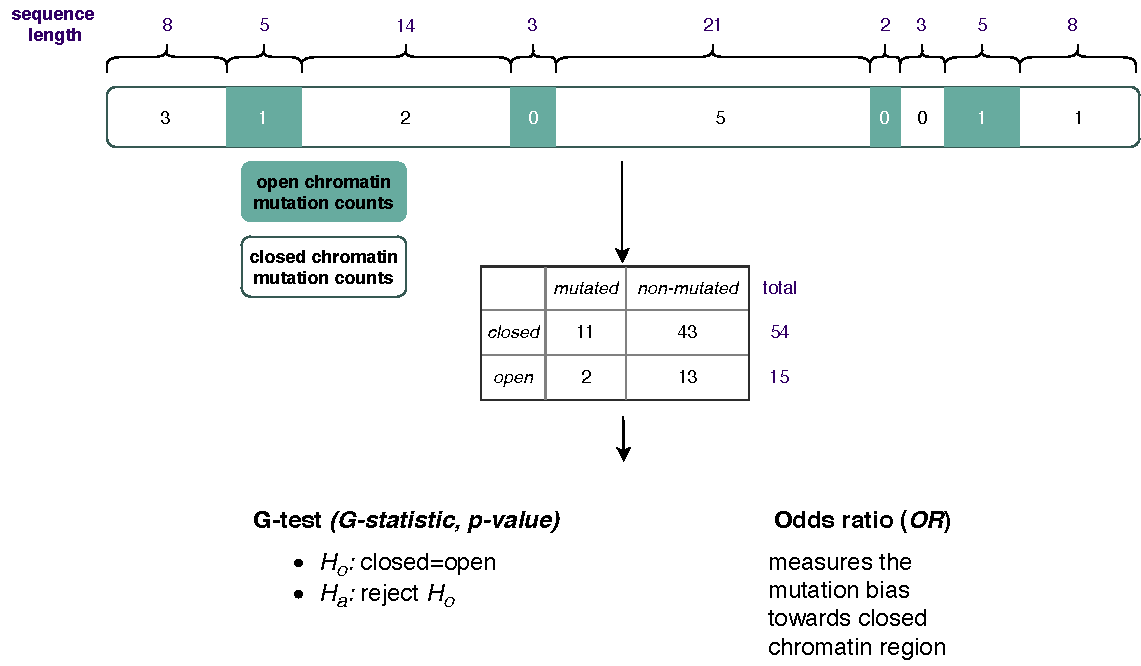
\includegraphics[scale=0.82]{graphics/mutdistribution.pdf}
\caption{}
    % \caption{\textbf{Establishing the relationship between cancer mutation and chromatin structure of the original cell type.} Mutations were sorted into open and closed regions to make a contingency table, from which a G-test can be performed and an Odds-ratio ($OR$) statistic can be calculated. The G-test establishes whether there is a significant bias in mutation location; $OR$ measures the degree of bias towards closed chromatin regions.}
    \label{fig:gle_workflow}
\end{figure}


\subsubsection{Homogeneity test for mutation location between closed and open regions}
I used the G-test of independence \citep{McDonald2014GtestStatistics} to examine the hypothesis whether the distribution of mutations are random across the genome - if this is the case, the expected number of mutations in the closed chromatin regions should not differ from that in the open regions. More formally:

\begin{itemize}
    \item $H_o (Null)$: Mutation abundance is independent of the chromatin status
    \item $H_a (Alternate)$: Mutation abundance is biased by the chromatin status
\end{itemize}

First, the expected number of observations for each cell was calculated as per Table \ref{tab:count_exp_demo}. For example, the expected number of mutated bases in the closed regions $e_i$ should be proportional to the number of bases available in the closed regions $c$ the number of mutations $m$. The departure of the observed count $o_i$ from the expected $e_i$ was measured by the $G$ statistic, calculated as:
\begin{equation}
    G = 2 \underset{i}{\sum} o_{i} \ln \frac{o_{i}}{e_{i}}
    \label{eq:g}
\end{equation}
where $o_{i}$ are observed values (\textit{i.e.} entries from Table \ref{tab:count_obs_demo}) and $e_{i}$ are expected values (\textit{i.e.} entries from Table \ref{tab:count_obs_demo}) and the p-value was obtained by permutation.

\vspace{0.2cm}
\begin{table}[ht!]
\caption{}
    % \caption{Demo contingency tables. Panel (a) contains the observed counts, each of the entries $c_m$, $c_n$, $o_m$ and $o_n$ represents an $o_i$ in equation \ref{eq:g}. Panel (b) contains the expected counts, each of the elements represents an $e_i$ in equation \ref{eq:g}.}
    \begin{subtable}[!h]{.5\textwidth}
        \centering
        \begin{tabular}{r|rr|r}
             & Mutated & Non-mutated & Total  \\
        \hline
            Closed & $c_m$ & $c_n$ & $c$ \\
            Open & $o_m$ & $o_n$ & $o$ \\
        \hline    
             & $m$ & $n$ & $t$ \\
        \end{tabular}
        \vspace{0.2cm}
    \subcaption{Observed counts}
    \label{tab:count_obs_demo}
    \end{subtable} 
    \quad % for side by side tables
    \begin{subtable}[!h]{.5\textwidth}
        \centering
        \begin{tabular}{r|rr|r}
             & Mutated & Non-mutated & Total  \\
        \hline     
            Closed & $c*m/t$ & $c*n/t$ & $c$ \\
            Open & $o*m/t$ & $o*n/t$ & $o$ \\
        \hline    
             & $m$ & $n$ & $t$ \\
        \end{tabular}
        \vspace{0.2cm}
    \subcaption{Expected counts}
    \label{tab:count_exp_demo}
    \end{subtable}    
\end{table}

\subsubsection{Odds ratio for the bias in GLE}
To complement the G-test, I used the odds ratio \citep[$OR$;][]{Hoppe2017OddsRatios} as a measure of preference for mutations to occur in closed chromatin regions compared to open regions. The formula for $OR$ of the contingency Table \ref{tab:count_obs_demo} is as follows:

\begin{equation}
    OR = \frac{c_m/c_n}{o_m/o_n}
    \label{eq:or}
\end{equation}

where $c_m$, $c_n$, $o_m$ and $o_n$ are all observed values that comes from Table \ref{tab:count_obs_demo}.

\subsubsection{Jackknife for the variation of $OR$}
It is worth noting that even within one cancer type, different donors might vary in the number of mutations they carry and the locations of the mutations. If a donor has a very distinctive mutation pattern, then it is probable that the $OR$ statistic for their whole cancer cohort mostly represents that donor only. To address this, I performed a jackknife analysis on this measure for each disease \citep{Miller1974TheReview}. An illustration of the jackknife workflow is shown in figure \ref{fig:jackknife_demo}. Specifically, to see how influential a donor is on the $OR$, one simply removes that donor and observes how $OR$ changes. If one applies that to every donor, one obtains a new set of $OR$ that reflects the potential range of the true $OR$.

\begin{figure}[h!]
    \centering
    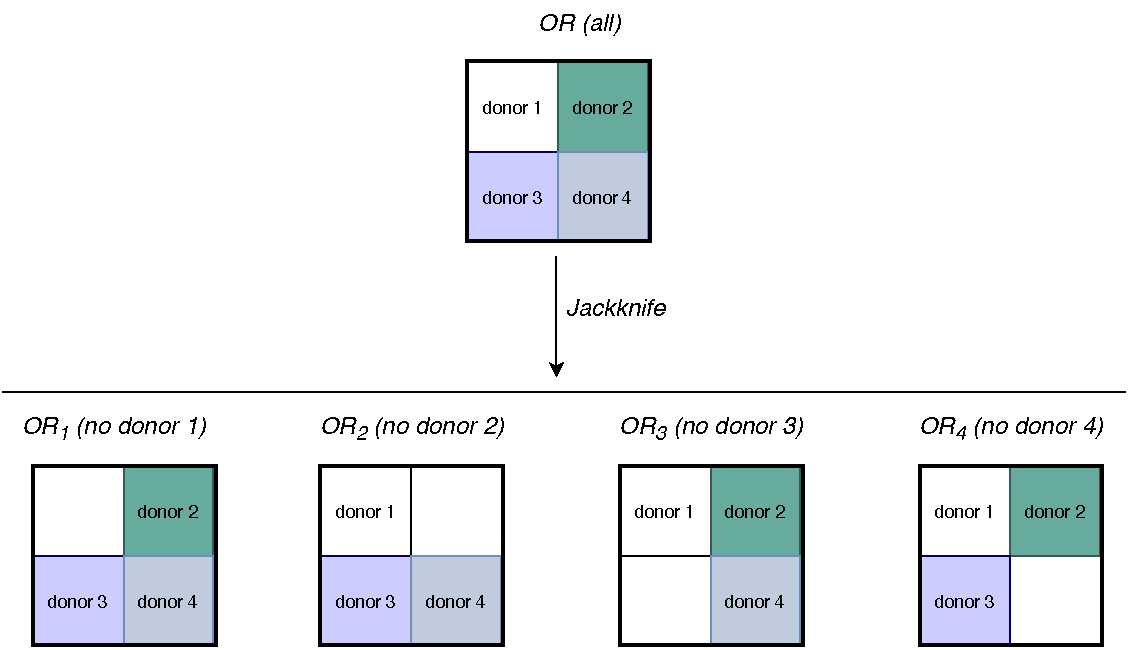
\includegraphics[scale=0.8]{graphics/jackknife_demo.pdf}
\caption{}
    % \caption{\textbf{Illustration of jackknife analysis}. For a hypothetical cancer with 4 donors, the original odds ratio $OR$ was computed. Donor 1 was then omitted and a new odds ratio $OR_1$ was recomputed and a pseudo value $OR^{pseudo}_1$ was obtained. The same was applied to every other donor. The end result was a set of odds ratio statistics $\{OR_1^{pseudo}, \ldots, OR_4^{pseudo}\}$ that were used to estimate the possible range of the true $OR$ statistic}
    \label{fig:jackknife_demo}
\end{figure}


\subsubsection{Shuffling DHS data}
It is a very natural concern that the calculation of $OR$ is itself biased towards closed chromatin regions due to its sheer large size compared to open regions. Besides, if chromatin status is a determinant of mutation location, then cells that have similar DHS should have somewhat similar GLE patterns. To address both of these, I shuffled the DHS data for the examined cancers. This means that, I sampled the PCAWG mutation data for each cancer. I then calculated the shuffled $OR$ - instead of sorting mutations by its own DHS data, I sorted mutations by the DHS data for all other cancers' original cells. Eventually, for each cancer, 11 shuffled $OR$'s were obtained. 

\subsection{Hypothesis testing of GLE between cancer pairs by bootstrap}

Following the attempt to investigate a suspected determinant of GLE, I examined whether GLE could discriminate cancers and what approaches to represent GLE could yield the most resolution. This includes the bin \textit{v.s.} smoothing representation and the Wasserstein \textit{v.s.} Euclidean distance measures. 

% add something about smooth vs bin and euclidean vs wasserstein

\subsubsection{Bin \textit{v.s.} smoothing representation}
\paragraph{Bin} As briefly described in Figure \ref{fig:mutdistribution_demo}, the bin representation segmented the genome into non-overlapping bins of 1 million base in length. The number of mutations in each bin was recorded for each chromosome, then divided by the total mutations in that chromosome to get the bin density. 
\paragraph{Smoothing} To address the issue with arbitrary boundaries introduced by the discrete bins approach, I proposed the smoothing representation that computes a sliding window of mutation density across each chromosome (Figure \ref{fig:mutdistribution_demo}). This was done using a kernel function \citep[equation \ref{eq:density};][]{Silverman1986DensityAnalysis}. The idea is that the density at a certain location $x$ should be proportional to the distance from $x$ to all other locations $X_i$ where mutations are observed. 

\begin{equation}
    \hat{f} = \frac{1}{nh} \underset{i=1}{\overset{n}{\sum}} K(\frac{x- X_i}{h})
    \label{eq:density}
\end{equation}

where $\hat{f}$ is the density for the location of interest $x$, $n$ is the total number of mutations, $X_i$'s are all genomic locations where mutations occur, $K$ is the kernel function - here the Gaussian kernel is used (appendix equation \ref{eq:gaussian}), $h$ is the bandwidth and determines the level of smoothing to be done - I used the canonical Scott's rule \citep[appendix equation \ref{eq:bandwidth};][]{Scott1992MultivariateEstimation} to determine the bandwidth. This is done using the python class \texttt{gaussian\_kde} from \texttt{scicy.stats}

\subsubsection{Euclidean \textit{v.s.} Wasserstein distance measure}
I separately used the Euclidean and Wasserstein distances for both representations to compare the GLE from two cancers. The basic difference between two is depicted in Figure \ref{fig:wasserstein_demo}. Intuitively, Euclidean measures the distance between two densities in a point-wise manner and in the vertical direction while Wasserstein uses both the vertical and horizontal directions. 

\paragraph{Euclidean} The Euclidean distance, also known as the Pythagorean distance is the most widely used distance. It is strictly the root sum of squares of the difference between each point on one density and its counterpart on the other density \citep[equation \ref{eq:euclid};][]{ONeill2006FrameFields}.

\begin{equation}
    d_E(a,b) = \sqrt{\sum_{i=1}^n (a_i - b_i)}
    \label{eq:euclid}
\end{equation}

where $d_E(a,b)$ is the distance between two densities $a$ and $b$; $a_i$ and $b_i$ are the elements of $a$ and $b$, respectively. This was executed by the python function \texttt{scipy.spatial.distance.euclidean}.

\paragraph{Wasserstein} It is reasonable to view mutation densities as masses of data spatially distributed across a 1-D axis (Figure \ref{fig:wasserstein_demo}). From this viewpoint, Wasserstein is a very appropriate measure of distance between two densities. Intuitively, it measures the minimal amount of work required to move mass from $A$ to $B$. Mathematically, it does so by searching for the minimum distance with respect to all the joint distributions $\gamma(x,y)$ of random variables $(X,Y)$ that have \glspl{marginal} $A$ and $B$\footnote{\textit{N.B.} There are infinite joint distributions $\gamma$}, as follows.

\begin{equation}
    d_W(A,B) = \underset{\gamma \in \mathcal{J}(A,B)}{\inf} \int |x-y| d \gamma(x,y) 
    \label{eq:wassertein}
\end{equation}

where $d_W$ is the Wasserstein distance; $\mathcal{J}$ is the set of all joint distributions $\gamma$. The $\gamma(x,y)$ terms represent the transport plans to move data from $A$ to $B$ and the $|x-y|$ term represents the distance to move from $A$ to $B$ based on that transport plan. The smallest value that takes into account the two terms (selected by the infimum function $\inf$) is the final Wasserstein distance. The assumption the Wasserstein distance imposes that $A$ and $B$ have the same masses was satisfied because by definition, the area under the curve for densities is always 1. This was done using the python function \texttt{scipy.stats.wasserstein\_distance}.

\begin{figure}[h!]
    \centering
    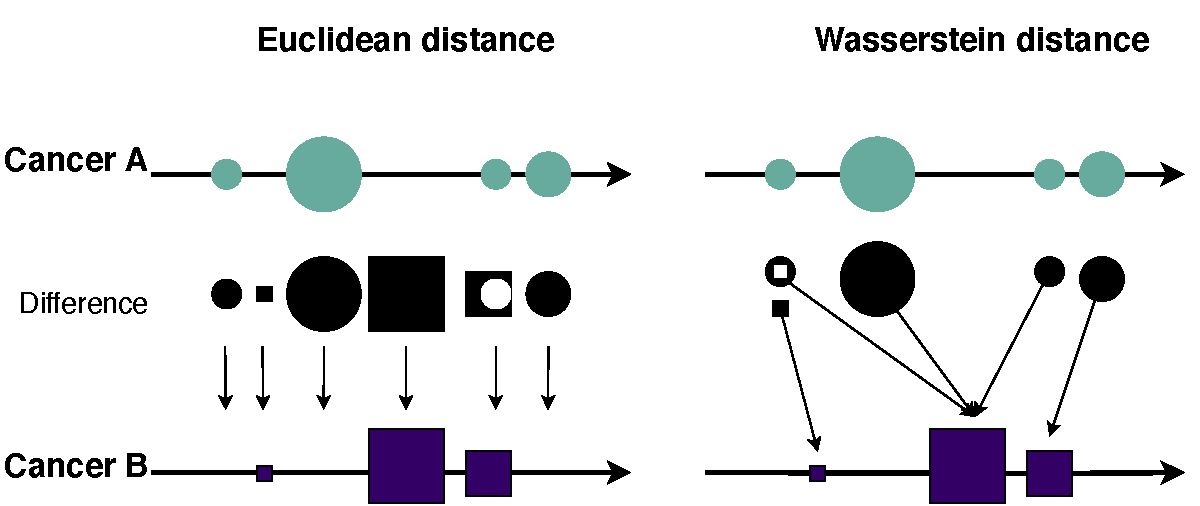
\includegraphics[scale=0.8]{graphics/wasserstein_demo.pdf}
    \caption{\textbf{Schematic diagram for Euclidean and Wasserstein distance between two vectors.} The green circles are data points on the GLE vector for Cancer A, the purple squares are data points on the GLE vector for Cancer B. The black shapes and the arrows combined represent the difference between Cancers A and B. Euclidean is the point-wise difference between the same location on vectors A and B, and is strictly in the vertical direction. In other words, the Euclidean distance between A and B only depends on how different points of similar coordinates are. Wasserstein takes into account both the vertical and horizontal directions; it is intuitively the minimal amount of work required to transport mass from A to B. The Wasserstein distance between A and B depends on both the difference between the magnitude of data points and the path it takes to move data points from A to B.}
    \label{fig:wasserstein_demo}
\end{figure}


\subsubsection{The bootstrap}

Having established the representations and distance measures, the next questions are whether the distance is significantly large enough to conclude that the cancer types have different patterns of GLE, and which representation can extract the most information for doing so. For this, I used the bootstrap method \citep{Singh2010BootstrapMethod}, which is based on random re-sampling. For a pair of cancers A and B, the formal hypotheses are

\begin{itemize}
    \item $H_o (Null)$ GLE for A is the same as B
    \item $H_a (Alternate)$ GLE for A is different from B
\end{itemize}

The bootstrap procedure is illustrated in Figure \ref{fig:bootstrap_demo}. For a pair of cancer types A and B with distance $d$, I first aggregated all mutations from the two cancers to create a pool of mutations. I then simulated 2 imaginary cancers 1 and 2 by randomly drawing mutations from that previously constructed mutation pool. The constraint on the simulation is that the total number of mutations in 1 has to be the same as either A or B - likewise for 2. This constraint is so that the simulated cancers are as close to the original as possible, so the result is not interfered by other factors than GLE. I then measured the simulated distance $d_i$ between 1 and 2. This process was repeated $n$ = 1000 times. To conclude that A and B are significantly different from each other, $d_{obs}$ should be larger than most of the simulated $d_i$. In the end, the proportion of the simulated distances that are greater than the observed distance between A and B is the estimated p-value the hypothesis test. 

\begin{figure}[h!]
    \centering
    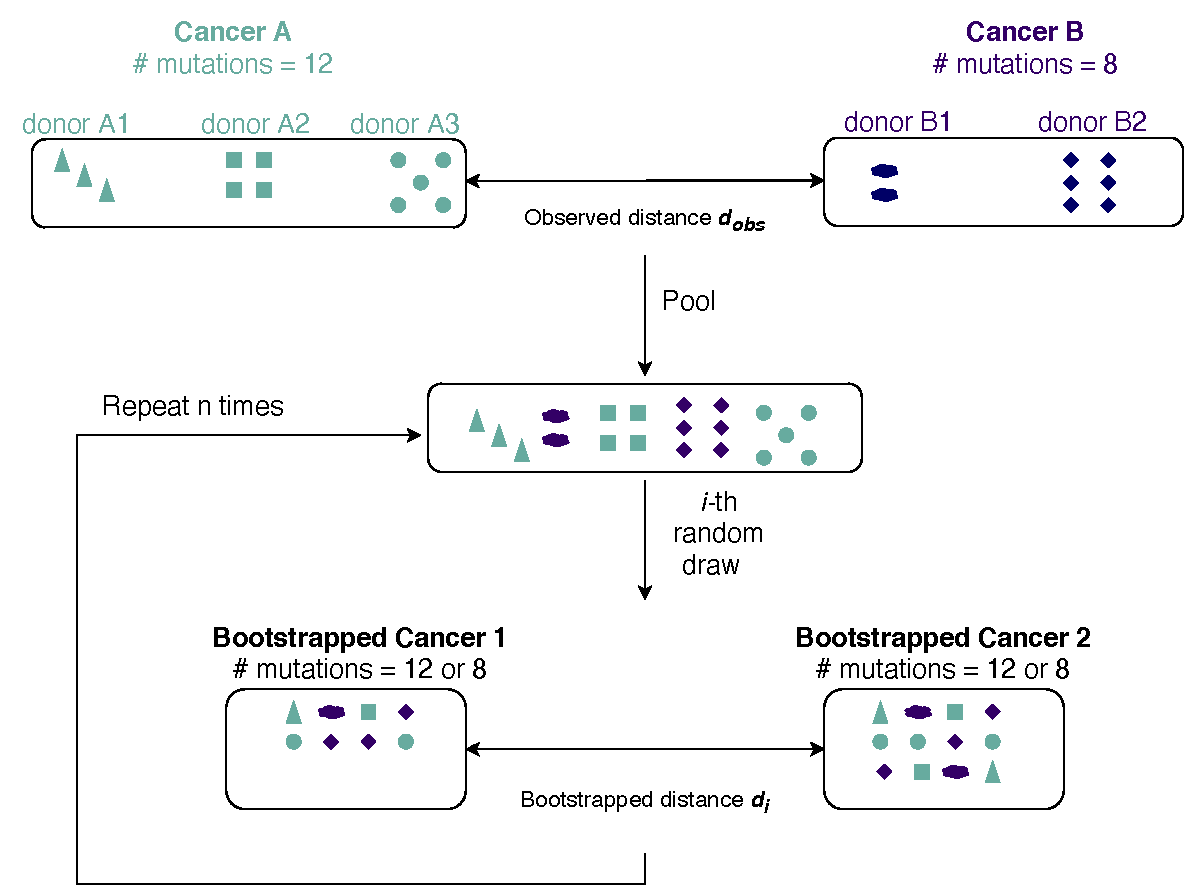
\includegraphics[scale=0.6]{graphics/bootstrap_demo.pdf}
    \caption{\textbf{Testing the hypothesis that two cancers share the same genomic distribution of mutations using bootstrap.} Mutations are pooled from 2 original cancers A and B, the distance between A and B is $d_{obs}$. 2 bootstrapped cancers 1 and 2 are then simulated by randomly drawing mutations from the pool, the number of mutations in 1 and 2 must be the same as either A or B. The distance $d_i$ between cancers 1 and 2 is then measured. This process is repeated 1000 times for each of the representations introduced. The estimated p-value is the number of times $d_i > d_{obs}$ divided by $n$.}
    \label{fig:bootstrap_demo}
\end{figure}


\section{Whole disease analysis of SCE}\label{methods:sce}
Cancers are known to have distinctive compositions of mutations, which themselves consist of two components: the base substitution and the flanking bases. Together, the two components are called sequence context effect (SCE). This section describes the statistical techniques  to measure the information content available in both components.

\subsection{Overview of the techniques to measure information}
The nature of SCE for both the base substitutions and the flanking bases is simply count data determined by categorical variables, which can be displayed on a contingency table. It is straightforward to assign this type of data to have a multinomial distribution. To establish or not one categorical variable (\textit{e.g.} the cancers) is deterministic of another (\textit{e.g.} the types of mutations), one could assume product multinomial sampling. Due to the mathematical connection between the product multinomial and Poisson distributions, one could execute this  via a generalised linear model (GLM) under the Poisson distribution \citep{Nelder1974LOGSQUARES.}. This project used the implementation previously developed in the Huttley lab, whose key function is \texttt{glm} from R \citep{Zhu2017}.

\subsubsection{Generalised linear model}
Table \ref{tab:glm_demo} illustrates how GLM can be used to evaluate whether one categorical variable is predictive of another. Specifically, the example tests whether the composition of base substitutions from the wildtype T differs for cancer A and B. Answering this question requires a null model ($H_o$) that assumes no relationship and a saturated model ($H_a$) that assumes a correlation between cancer types ($\lambda_{cancer}$) and the substitution types ($\lambda_{sub}$). This correlation manifests through the $\lambda_{cancer:sub}$ that is present in $H_a$ but absent in $H_o$. By measuring the deviance statistic $D$ (equation \ref{eq:deviance}), \textit{i.e.} how much information the null is missing from the saturated model, and contrasting $D$ against the $\chi^2$ distribution, a p-value can be obtained. A small enough p-value (usually $<0.05$) means that $\lambda_{cancer}$ is predictive of $\lambda_{sub}$.

\begin{equation}
D = -2 \ln \frac{\hat{L}(saturated)}{\hat{L}(null)}
\label{eq:deviance}
\end{equation}
where $D$ is the deviance statistic; $\hat{L}$ is the estimated maximum likelihood for the parameters in the corresponding models.

\begin{figure}[h!]
  \begin{minipage}[c]{0.5\textwidth}
    \captionof{table}{\textbf{Example of how GLM and RE can be used for categorical data in a contingency table}. In this example, the categorical variable for cancer type $\lambda_{cancer}$ takes values cancer A or cancer B; the variable for the composition of base substitution $\lambda_{sub}$ takes values T$\rightarrow$A, T$\rightarrow$C and T$\rightarrow$G. To establish whether $\lambda_{cancer}$ is explanatory of $\lambda_{sub}$, one can perform a hypothesis test based on a null and a saturated model (formulae \ref{eq:spectra_demo}; the $counts$ corresponds to the $count$ term in equation \ref{eq:spectra_demo}). The hypothesis test outputs a p-value; if p-value is small enough, it can the explanatory relationship. The test also allows estimating $RE$, which measures how much information is contributed by each entry in the table.} 
    \label{tab:glm_demo}
  \end{minipage}\hfill
  \begin{minipage}[c]{0.48\textwidth}
    \begin{tabulary}{\columnwidth}{rRRR}
    \toprule
        & \textbf{T$\rightarrow$A} & \textbf{T$\rightarrow$C} & \textbf{T$\rightarrow$G}  \\
    \hline
        \textbf{Cancer A} & $count_{T>A}$ & $count_{T>C}$ & $count_{T>G}$  \\
        \textbf{Cancer B} & $count_{T>A}$ & $count_{T>C}$ & $count_{T>G}$  \\
    \bottomrule
    \end{tabulary}
    \vspace{1cm}
    \begin{equation}
        \begin{aligned}
            H_o: \ln{count} =& \lambda_{cancer} + \lambda_{sub}  & \\
            H_a: \ln{count} =& \lambda_{cancer} + \lambda_{sub} + \lambda_{cancer:sub}
        \end{aligned}
        \label{eq:spectra_demo}
    \end{equation}
  \end{minipage}
\end{figure}


\subsubsection{Relative entropy}\label{methods:re}
To measure the amount of information contributed by each entry in the contingency table ($count$ in Table \ref{tab:glm_demo}), one use relative entropy ($RE$). $RE_i$ for the entry $i$ can be calculated via the deviance residual $r_i$ of the entry (appendix equation \ref{eq:dev_res}). Note that while the deviance $D$ measures the departure of the null from the saturated, $r_i$ is the contribution from entry $i$ to this departure, and the sum of all $r_i^2$ is equal to $D$. The reason why I chose $RE$, not deviance residual, to be the measure of information is because it scales the data by its sample size, thereby making comparison across different hypothesis tests valid. It is calculated as follows

\begin{equation}
    RE_i = \frac{r_i}{2n} 
    \label{eq:re}
\end{equation}

where $RE_i$ is the relative entropy for entry $i$ of the contingency table; $r_i$ is its deviance residual and $n$ is the total counts. 

\subsection{Base substitutions}
\subsubsection{Composition of base substitutions for individual cancers}
To examine the patterns of base substitution in a cancer, I calculated the $RE$'s when comparing that cancer to a ``null cancer'', where all mutation counts are the same (Table \ref{tab:glm_spectra}). Due to the difference in the abundance of nucleotides (\textit{e.g.} only 41\% of the human genome is CG, the rest is AT; the unbalance is potentially even greater when only one DNA strand is considered), I separately calculated four $RE$ sets for substitutions that involved different wildtype bases. Table \ref{tab:glm_spectra} illustrates the set whose wildtype base is T. 

\vspace{0.2cm}
\begin{figure}[h!]
  \begin{minipage}[c]{0.4\textwidth}
    \captionof{table}{\textbf{Contingency table to examine the composition of base substitutions in Cancer A}. Cancer A is compared to a null cancer where all counts are the same. The resulting $RE$'s represent the excess/deficit of certain substitutions. This particular table computes the $RE$ set for substitutions whose wildtype is T. $\lambda_{cancer}$ is a categorical variable taking values \textbf{Cancer A} or \textbf{Null}. $\lambda_{sub}$ indicates whether the counted substitution is \textbf{T$\rightarrow$A}, \textbf{T$\rightarrow$C} or \textbf{T$\rightarrow$G}. For each cancer, three similar tables are required for substitutions of A, C and G.} 
    \label{tab:glm_spectra}
  \end{minipage}\hfill
  \begin{minipage}[c]{0.59\textwidth}
    \begin{tabulary}{\columnwidth}{lCCCR}
    \toprule
        & \textbf{T$\rightarrow$A} & \textbf{T$\rightarrow$C} & \textbf{T$\rightarrow$G}  & \textbf{total} \\
    \hline
        \textbf{Cancer A} & $count_{T>A}$ & $count_{T>C}$ & $count_{T>G}$ & $count_{tot}$ \\
        \textbf{Null} & $count_{tot}/3$ & $count_{tot}/3$ & $count_{tot}/3$ & $count_{tot}$ \\
    \bottomrule
    \end{tabulary}
    \vspace{0.9cm}
    \begin{equation}
        \begin{aligned}
            H_o: \ln{count} =& \lambda_{cancer} + \lambda_{sub}  & \\
            H_a: \ln{count} =& \lambda_{cancer} + \lambda_{sub} + \lambda_{cancer:sub}
        \end{aligned}
        \label{eq:spectra}
    \end{equation}
  \end{minipage}
\end{figure}


I visualised $RE$ for a cancer in the form of sequence logo plot. Each row of the plot corresponds to a model of a wildtype base, where the heights of the letters are the $RE$'s, which represent whether there is an abnormal excess/deficit of certain mutations in that cancer and the level of this abnormality.

\subsubsection{Base substitutions across cancers}
Having looked at the base substitutions for individual cancers, I examined how well base substitutions can be used to discriminate cancers. To compare two cancers, the contingency table for this analysis is similar to the example in Table \ref{tab:glm_demo}. Similar to the case of individual cancers, I analysed mutations from different wildtype bases separately. In addition to the $RE$'s, also looked at the p-values from the hypothesis tests. Since there are four hypothesis tests, there are four p-values, which I combined these p-values into one p-value using the Fisher's method \citep[details in \ref{apdx:fisher};][]{Fisher1992StatisticalWorkers}. Briefly, Fisher's method adds up all the logs of the member p-values, this value is doubled and contrasted against the $\chi^2$ distribution to obtain the final joint p-value.

\subsection{Flanking bases}
In the subsection, we are interested in the information content available in the flank base component of SCE, including positions -1, +1, -2 and +2 with respect to the mutation. Analogically to the base substitution, I separated the analysis for different mutations due to their different frequencies of occurrence. Figure \ref{fig:nbr_demo} illustrates how how information can be measured for position +1 of the C$\rightarrow$T mutation in some cancer A. Specifically, the analysis measures the extent to which bases found next to the C$\rightarrow$T mutation tend to differ from bases next to a randomly selected C in the genome. To do this, for each C$\rightarrow$T I randomly selected a C in the genome and recorded the base at position +1. I then received a contingency table. Using the models in formulae \ref{eq:nbr_demo}, I obtained the $RE$'s, as described in subsection \ref{methods:re}, whose total is the desired measure of information. I measured the total $RE$ for all other flank positions of the 5-mer context and all other mutations.

\begin{figure}[h!]
  \begin{minipage}[c]{0.48\textwidth}
    \caption{
      \textbf{The smoothing approach is expected to be more robust than the bin approach.} Both panels depict the same mutation location data for a hypothetical chromosome, with the black dots below the x-axis representing the true location of mutations. By binning the genome by convention, one counts the number of mutations in each green bin. The obtained GLE data is then the green dots on top of each bin. This binned GLE data changes when shifting the bin boundaries from panel (a) to panel (b). On the contrary, the smooth representation of GLE, which adopts \gls{density} estimation, is depicted by the purple dots on the purple line. By smoothing the genome, GLE data is the same for both panels. 
    } \label{fig:mutdistribution_demo}
  \end{minipage}\hfill
  \begin{minipage}[c]{0.55\textwidth}
    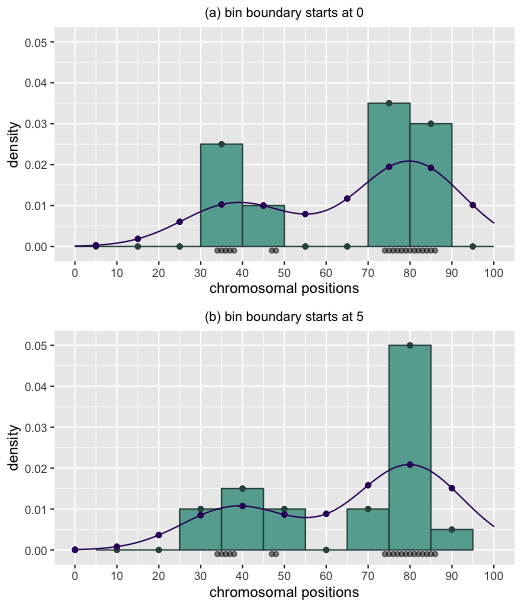
\includegraphics[width=\textwidth]{graphics/mutdistribution_demo.png}
  \end{minipage}
\end{figure}


\section{Mutation-based classifier for cancers}\label{methods:ml}
Based on the premise that GLE and SCE are important aspects of a cancer mutation profile, this section explores how we could exploit the information from GLE and SCE for cancer classification. Because I trialled different approaches to represent data, I expect the known properties of the best performing approach should reveal important characteristics of the data. More critically, it should validate the findings from whole disease analyses, thereby consolidating our understanding of cancer mutagenesis.

\subsection{Machine learning workflow}
The fundamental value of a classifier is that it can be used to predict data not previously seen by the classifier. As such, for all classifiers trained in the subsequent subsections, I followed the same training procedures, as follows. 

\subsubsection{K-nearest neighbours}
Because I used pairwise distances between observations to describe both GLE and SCE, I use K-nearest neighbours \citep[KNN;][]{Neath2010DiscriminationClassification}, a distance-based algorithm, to train the classifier. There are two reasons there was a preference for distances over raw parameters. First, as in the case for most biological data, our data suffers from the curse of dimensionality \citep{Banks2003DataStatistics}, meaning there are more parameters than there are observations, making inference less robust. For example, the bin representation for GLE alone has about 3000 parameters corresponding to 3000 bins, while there are only about hundreds of donors available. Describing data in terms of distances is therefore a way to escape the curse of dimensionality. Second, I was interested in experimenting with different types of metrics that might better describe the data than the typically default Euclidean distance. The principle of the KNN algorithm is straightforward (Figure \ref{fig:knn_demo}): when prediction on an unknown donor needs to be made, KNN calculates the distances from the unknown to all known donors in the training set and identifies the nearest training points (known neighbours) to the unseen donor. The predicted cancer will be the predominant cancer within these neighbours.

\subsubsection{F1-score}
\subsubsection{Cross validation}

\subsection{Classifier by GLE}
\subsection{Classifier by SCE}
\subsection{Combining GLE with SCE in a joint classifier}
